% This file was created by matlab2tikz.
%
%The latest updates can be retrieved from
%  http://www.mathworks.com/matlabcentral/fileexchange/22022-matlab2tikz-matlab2tikz
%where you can also make suggestions and rate matlab2tikz.
%
\definecolor{mycolor1}{rgb}{0.00000,0.44700,0.74100}%
%
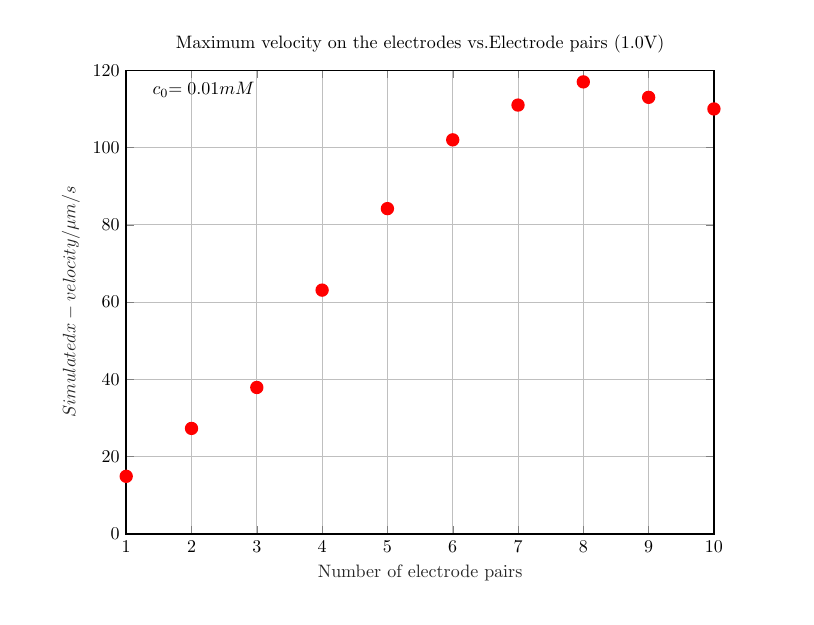
\begin{tikzpicture}[scale=0.65]

\begin{axis}[%
thick,
width=4.521in,
height=3.566in,
at={(0.758in,0.481in)},
scale only axis,
xmin=1,
xmax=10,
xlabel style={font=\color{white!15!black}},
xlabel={Number of electrode pairs},
ymin=0,
ymax=120,
ylabel style={font=\color{white!15!black}},
ylabel={$\text{Simulated x-velocity / }\mu\text{m/s}$},
axis background/.style={fill=white},
title={Maximum velocity on the electrodes vs.Electrode pairs (1.0V)},
xmajorgrids,
ymajorgrids
]
\addplot [color={red}, only marks, mark size=3.3pt, mark=*, mark options={solid, red}, forget plot]
  table[row sep=crcr]{%
1	14.9\\
2	27.3\\
3	37.9\\
4	63.1\\
5	84.2\\
6	102\\
7	111\\
8	117\\
9	113\\
10	110\\
};
\node[right, align=left]
at (axis cs:1.3,115) {$\text{c}_\text{0}\text{ = 0.01mM}$};
\end{axis}

\begin{axis}[%
width=5.833in,
height=4.375in,
at={(0in,0in)},
scale only axis,
xmin=0,
xmax=1,
ymin=0,
ymax=1,
axis line style={draw=none},
ticks=none,
axis x line*=bottom,
axis y line*=left
]
\end{axis}
\end{tikzpicture}%